% !TEX root = main.tex
\section{Measures}
\label{sec:measures}
In this section we now present the different measures adopted to evaluate the goodness of our goals.

The first measure we are interested in is the \emph{regularity} of the sequence of taps performed by the user. Moreover it is interesting to measure also the frequency synchronization w.r.t. the given beat and the synchronization ratio, i.e. the ratio between the mean of tap intervals and the given soundtrack's beat distance.
Let us now see how we defined such measures.
\subsection{Regularity}
For regularity we mean that the user should tap on the balloon at regular intervals. So a good regularity measure should be better when the time intervals are very similar to each other and bad when they are not. Therefore we decided to measure regularity as the \emph{mean squared error} (MSE) of the intervals between each user's tap.
The lower the error the better the regularity.
Thus the mathematical formulation then is
\begin{align}
	\frac{1}{n}\displaystyle\sum\limits_{i=0}^n(\bar{X}-X_i)^2
\end{align}
where $X_i$ is the ith time interval and $\bar{X}$ is the mean of the time intervals.

It is worth to notice that the regularity could be uncorrelated to the synchronization, in the sense that a user could produce a very regular sequence without being synchronized with the provided soundtrack.

\subsection{Synchronization}
As stated above the regularity might be uncorrelated to the synchronization, so we also want to have a measure of how well the user is synchronized with the provided soundtrack.
In order to achieve this, we measure for each beat interval the delay between the user's tap and the last closest beat.
If no user's tap or more than one occur in the interval, we take the whole distance between two consecutive beat as delay.

\begin{figure}[h!t]
\label{fig:sync-measure}
\centering
	{\setlength{\fboxsep}{1.5pt}
	 \fbox{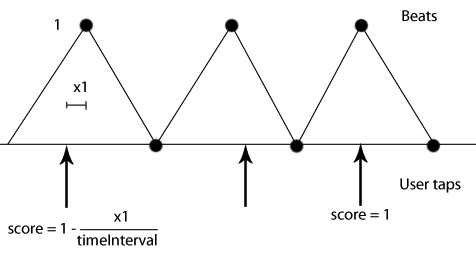
\includegraphics[width=0.45\textwidth]{sync}}}
\caption{The synchronization measure}
\end{figure}

We then take the sum of every delay as the final measure, therefore the lower the sum the better the overall synchronization.

\subsection{Synchronization Ratio}
As we already stated, the user could be regular without being synchronized with the background music. However it may happen that the user is synchronized to a tempo which is $n$ times faster or slower than the given one.
In order to discover such a synchronization we decided to measure the ratio between the average time interval between user's taps and the regular interval of the soundtrack. The mathematical formalization for this is the following:
\begin{align}
	SyncRatio = \frac{\bar{X}}{T}
\end{align}
where $\bar{X}$ is the average time interval between user's taps and T is the interval between the soundtrack's beats.
If the number is close to an integer number and the user's sequence is regular then the user is likely synchronized to a multiple (or divisor) of the given tempo.